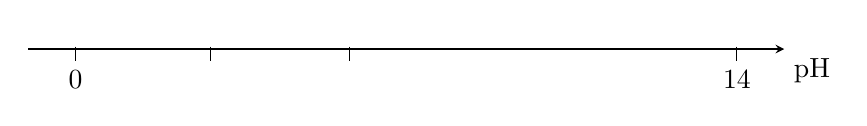
\begin{tikzpicture}[scale=0.6]
\coordinate (O) at (-1,0);
\coordinate (X) at (15,0);
\coordinate (P1) at (2.85,0.05);
\coordinate (P2) at (5.80,0.05);
\coordinate (A1) at (1.425,0.05);
\coordinate (A2) at (4.325,0.05);
\coordinate (A3) at (9.9,0.05);
\coordinate (P0) at (0,0.05);
\coordinate (P14) at (14,0.05);
 
 \draw[->, >=stealth] (O) -- (X) node[below right]{\textrm{pH}};
 \draw (P1) --++(0,-0.3) node[below]{\reponseX{}};
 \draw (P2) --++(0,-0.3) node[below]{\reponseY{}};
 \draw (A1) node[above]{\reponseA{}};
 \draw (A2) node[above]{\reponseB{}};
 \draw (A3) node[above]{\reponseC{}};
\draw (P0) --++(0,-0.3) node[below]{$0$};
\draw (P14) --++(0,-0.3) node[below]{$14$};

\end{tikzpicture}
